%!TeX root = main.tex
\chapter{Beispiel}

\section{Allgemein} \label{sec:allgemeinProblem}
\begin{comment}
sei $\phi\in\{\frac{1}{t^k},\frac{1}{t^2}+\frac{1}{t^3},\dots\}$
\begin{enumerate}
\item Starte mit: $P(t,\partial_t):=(\partial_t-\frac{d}{dt}\phi(t)) \cdot
\mbox{Hauptnenner }\in\C[t]<\partial_t>$
\item Furiertrafo: $F_P(z,\partial_z)=P(\partial_z,-z)\in\C[z]<\partial_z>$
\item $x=z^{-1}$ und $\partial_x=-z^2\partial_z$ \\
\[
Q(x,\partial_x):=F_P(x^{-1},-x^2\partial_x)\cdot \mbox{Hauptnenner
}\in\C[x]<\partial_x>
\]
\item Berechne für $Q$ das NP usw...
\end{enumerate}
\end{comment}

Hier wollen wir nun eine Spezielle Klasse von Meromorphen Zusammenhängen, die
die durch das folgende Rezept entstehen.
\begin{enumerate}
\item Wähle ein $\phi$ zB. aus
$\{\frac{1}{t^k},\frac{1}{t^2}+\frac{1}{t^3},\dots\}$
\item und beginne dann mit
\[
\tilde P(t,\partial_t):=(\partial_t-\frac{d}{dt}\phi(t))
\]
\item Multipliziere mit Hauptnenner
\[
P(t,\partial_t):=(\partial_t-\frac{d}{dt}\phi(t)) \cdot
\mbox{Hauptnenner }\in\C[t]<\partial_t>
\]
\item wende auf $P$ die Fouriertransformation 
$F_P(z,\partial_z)=P(\partial_z,-z)$ an und erhalte ein Element
in $\C[z]<\partial_z>$
\item Wende die Übergänge $x=z^{-1}$ und $\partial_x=-z^2\partial_z$ an 
\[
\tilde Q(x,\partial_x):=F_P(x^{-1},-x^2\partial_x)
\]
\item Multipliziere mit Hauptnenner
\[
Q(x,\partial_x):=F_P(x^{-1},-x^2\partial_x)\cdot \mbox{Hauptnenner
}\in\C[x]<\partial_x>
\]
\end{enumerate}

\begin{comment}
warum sind diese wichtig??
\end{comment}

\section{Explizit}
Betrachte nun Spezialfälle von \ref{sec:allgemeinProblem}.

Im besonderen zunächst $\cD/\cD(x^3\partial_x^2+1)$ also mit
$P=x^3\partial_x^2+1$

\begin{figure}[H]
\label{fig:Exmp-A}
%\caption{Zu Beispiel \ref{exmp:Exmp-A}}
\begin{center}
\fbox{
  \subfloat[Newton Polygon zu\\ $P=x^3\partial_x^2+1$]{
    \label{fig:Exmp-A-1}
    \begin{tikzpicture}[scale=1.5]
    \def\myPoints{{(0,0)}, {(2,1)}}
    \def\myPath{(-.5,0) -- (0,0) -- (2,1) -- (2,3)}
    \myNewtonPlot{\myPoints}{\myPath}{2}{0}{3}{
      $N(P)$
    }
    \end{tikzpicture}
  }
  \quad
  \subfloat[Newton Polygon zu\\ $\rho^+P$]
  {
    \label{fig:Exmp-A-2}
    \begin{tikzpicture}[scale=1.5]
    \def\myPoints{{(0,0)}, {(2,2)}}
    \def\myPath{(-.5,0) -- (0,0) -- (2,2) -- (2,3)}
    \myNewtonPlot{\myPoints}{\myPath}{2}{0}{3}{$N(\rho^+P)$}
    \end{tikzpicture}
  }
}
\end{center}
\end{figure}

% vim: set ft=tex :
